\hypertarget{haftpflichtrecht}{%
\section{Haftpflichtrecht}\label{haftpflichtrecht}}

\hypertarget{formen}{%
\subsection{Formen}\label{formen}}

\textbf{Verschuldungshaftung:} Schädiger haftet grundsätzlich nur, wenn
er den Eintritt des Schadens verschuldet hat (Persönliche
Vorwerfbarkeit)

\textbf{Kausalhaftung:} Setzt kein Verschulden voraus, sondern ist
gegeben, wenn durch das Gesetz festgelegte Tatbestandsvoraussetzungen
erfüllt sind.

\begin{itemize}
\tightlist
\item
  einfache Kausalhaftung
\item
  Geschäftsherrenhaftung (Art. 55 OR) - Chef haftet für Mitarbeiter
\item
  Werkeigentümerhaftung (Art. 58 OR) - Haft für Werke (Baugerüste,
  Häuser, \ldots{})
\item
  Haftung des Grundeigentümers (Art. 679 ZGB)
\item
  Produktehaftpflicht (PrHG)
\item
  Gefährdungshaftung: Bestimmten Einrichtungen sind Gefahren inhärent,
  die den Betreibern dieser Einrichtungen eine besondere Verantwortung
  aufbürden (Gefahrensatz).
\end{itemize}

\hypertarget{voraussetzungen}{%
\subsection{Voraussetzungen}\label{voraussetzungen}}

\begin{itemize}
\tightlist
\item
  Schaden
\item
  Widerrechtlichkeit
\item
  Adäquater Kausalzusammenhang
\item
  Verschulden
\end{itemize}

\begin{figure}
\centering
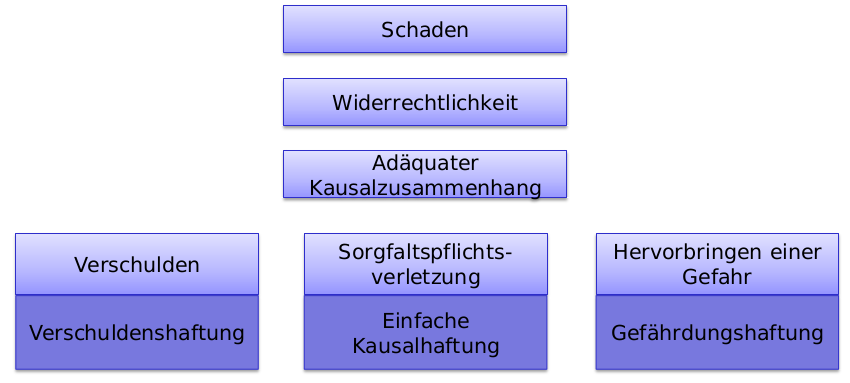
\includegraphics{figures/haftpflichtVerschulden.png}
\caption{Voraussetzungen bei Verschuldens- und Kausalhaftung}
\end{figure}

\hypertarget{definition-schaden}{%
\subsubsection{Definition Schaden}\label{definition-schaden}}

Unfreiwillige Verminderung des Vermögens in Form: - Abnahme der Aktiven
- Zunahme der Passiven - Entgangener Gewinn

\emph{Der Schaden als Vermögenseinbusse bestimmt sich grundsätzlich nach
der Differenz zwischen dem gegenwärtigen Vermögensstand und dem Stand,
den das Vermögen ohne das schädigende Ereignis hätte.}

\hypertarget{schadensformen}{%
\subsubsection{Schadensformen}\label{schadensformen}}

\begin{itemize}
\tightlist
\item
  Vermögensschaden

  \begin{itemize}
  \tightlist
  \item
    Definition von vorher: Schaden als Vermögenseinbusse
  \end{itemize}
\item
  Personenschaden

  \begin{itemize}
  \tightlist
  \item
    Beeinträchtigung der Gesundheit einer Person
  \end{itemize}
\item
  Sachschaden

  \begin{itemize}
  \tightlist
  \item
    Wenn eine Sache Schaden nimmt, wie z.B. ein Laptop
  \end{itemize}
\item
  Immaterieller Schaden

  \begin{itemize}
  \tightlist
  \item
    Reputation
  \item
    Persönlichkeitsverletzung
  \end{itemize}
\item
  Direkter Schaden

  \begin{itemize}
  \tightlist
  \item
    Der Schaden ist durch das schädige Ereignis direkt ausgelöst
  \end{itemize}
\item
  Indirekter Schaden

  \begin{itemize}
  \tightlist
  \item
    Der Schaden ensteht später als das schädigende Ereignis
  \end{itemize}
\end{itemize}

\hypertarget{wiederrechtlichkeit}{%
\subsubsection{Wiederrechtlichkeit}\label{wiederrechtlichkeit}}

\begin{itemize}
\tightlist
\item
  Es muss entweder ein absolutes Recht verletzt sein

  \begin{itemize}
  \tightlist
  \item
    Absolute Rechte sind Rechte, die gegenüber allen gelten

    \begin{itemize}
    \tightlist
    \item
      Besitz / Eigentum
    \item
      Leben
    \item
      Ehre
    \item
      Gesundheit
    \end{itemize}
  \end{itemize}
\item
  Oder es muss eine Schutznom verletzt werden

  \begin{itemize}
  \tightlist
  \item
    Veruntreuung oder Datenbeschädigung
  \end{itemize}
\end{itemize}

\textbf{Datenbeschädigung} Wer unbefugt elektronisch oder in
vergleichbarer Weise gespeicherte oder übermittelte Daten verändert,
löscht oder unbrauchbar macht, wird, auf Antrag, mit Freiheitsstrafe bis
zu drei Jahren oder Geldstrafe bestraft.

\hypertarget{widerrechtlichkeit---rechtfertigungsgruxfcnde}{%
\subsubsection{Widerrechtlichkeit -
Rechtfertigungsgründe}\label{widerrechtlichkeit---rechtfertigungsgruxfcnde}}

\begin{itemize}
\tightlist
\item
  Notwehr (Art. 52.1 OR) - Verhältnissmässige Abwehr in einer
  Notsituation
\item
  Notstand (Art. 52.2 OR) - Um sich selber zu schützen, greift man in
  das Rechtsgut eines anderen ein.
\item
  Selbsthilfe (Art. 52.3 OR) - Die eigene Sache darf wieder veschaft
  werden (ohne Selbstjustiz)
\item
  Einwilligung des Verletzten - z.B. eine Operation
\item
  Amtspflicht - z.B. Taschenkontrolle durch einen Polizisten
\end{itemize}

\hypertarget{aduxe4quater-kausalzusammenhang}{%
\subsubsection{Adäquater
Kausalzusammenhang}\label{aduxe4quater-kausalzusammenhang}}

\begin{itemize}
\tightlist
\item
  Wenn eine Ursache geeignet ist, eine Wirkung zu erbringen.
\end{itemize}

\hypertarget{verschuldungsformen}{%
\subsubsection{Verschuldungsformen}\label{verschuldungsformen}}

\begin{itemize}
\tightlist
\item
  \textbf{Vorsatz}: Der Schuldner strebt einen Erfolg bewusst an.
\item
  \textbf{Eventualvorsatz}: Der Schädiger nimmt ein Schaden in Kauf.
\item
  \textbf{Fahrlässigkeit}: Nicht absichtlich angestrebte
  \emph{mangelhafte Sorgfalt} führt zur Verletzung.

  \begin{itemize}
  \tightlist
  \item
    \textbf{Grobe Fahrlässigkeit}: Die gebotene Sorgfaltspflicht ist in
    besonders schwerer Weise verletzt.
  \item
    \textbf{Leichte Fahrlässigkeit}: Das Verhalten des Schädigers kann
    als ``einigermassen verständlich'' bezeichnet werden. z.B. wenn man
    aus Versehen jemand mit einer Dampfwalze überfährt
  \end{itemize}
\end{itemize}
